\documentclass{beamer}
%
% Choose how your presentation looks.
%
% For more themes, color themes and font themes, see:
% http://deic.uab.es/~iblanes/beamer_gallery/index_by_theme.html
%
\mode<presentation>
{
  \usetheme{default}      % or try Darmstadt, Madrid, Warsaw, ...
  \usecolortheme{crane} % or try albatross, beaver, crane, ...
  \usefonttheme{structurebold}  % or try serif, structurebold, ...
  \setbeamertemplate{navigation symbols}{}
  \setbeamertemplate{caption}[numbered]
} 

\usepackage[english]{babel}
\usepackage[utf8x]{inputenc}

\title[ML]{Machine Learning}
\author{Pawel Wocjan}
\institute{University of Central Florida}
\date{Spring 2019}

\begin{document}

\begin{frame}
  \titlepage
\end{frame}

\begin{frame}{Sources for Slides}

\begin{itemize}
\item I have extensively used the machine learning materials that have been prepared by Google. 

\medskip
\footnotesize{ 
\url{https://developers.google.com/machine-learning/crash-course/}
}

\item Google has licensed these materials under the Creative Commons Attribution 3.0 License.

\medskip
\footnotesize{ 
\url{https://creativecommons.org/licenses/by/3.0/}
}
\end{itemize}
\end{frame}

% Uncomment these lines for an automatically generated outline.
\begin{frame}{Outline}
  \tableofcontents
\end{frame}

\section{Framing}

\subsection{ML Terminology}

\begin{frame}{ML Terminology}

\begin{itemize}
\item What is (supervised) machine learning? Concisely put, it is the following:

\medskip
\emph{ML systems learn how to combine input to produce useful predictions on never-before-seen data.}

\item Let's explore fundamental machine learning terminology.
\end{itemize}
\end{frame}

%%%

\begin{frame}{ML Terminology}

\begin{itemize}
\item 
A {\bf label} is the thing we're predicting -- the $y$ variable in simple linear regression. The label could be the future price of wheat, the kind of animal shown in a picture, the meaning of an audio clip, or just about anything.

\item 
A {\bf feature} is an input variable — the $x$ variable in simple linear regression. 

\item A simple machine learning project might use a single feature, while a more sophisticated machine learning project could use millions of features, specified as:   
\[
x_1,x_2,\ldots,x_n
\]
\end{itemize}

\end{frame}

%%%

\begin{frame}{ML Terminology}

\begin{itemize}
\item In the spam detector example, the features could include the following:
\begin{itemize}
\item words in the email text
\item sender's address
\item time of day the email was sent
\item email contains the phrase "one weird trick."
\end{itemize}

\item An {\bf example} is a particular instance of data, $x$. We break examples into two categories:
\begin{itemize}
\item
labeled examples

\item
unlabeled examples
\end{itemize}
\end{itemize}

\end{frame}

%%%

\begin{frame}{ML Terminology}

\begin{itemize}
\item A {\bf labeled example} includes both feature(s) and the label. That is:

\medskip
\texttt{labeled example: \{features, label\}}: $(x, y)$

\item We use labeled examples to train the model. In our spam detector example, the labeled examples would be individual emails that users have explicitly marked as "spam" or "not spam."

\item 
An {\bf unlabeled example} contains features but not the label. That is:

\medskip
\texttt{unlabeled example: \{features, ?\}}: $(x, ?)$

\item Once we've trained our model with labeled examples, we use that model to predict the label on unlabeled examples. In the spam detector, unlabeled examples are new emails that humans haven't yet labeled.
\end{itemize}

\end{frame}

\begin{frame}{ML Terminology}
\begin{itemize}
    \item A model defines the relationship between features and label. For example, a spam detection model might associate certain features strongly with "spam". Let's highlight two phases of a model's life:
    \begin{itemize}
        \item {\bf Training} means creating or learning the model. That is, you show the model labeled examples and enable the model to gradually learn the relationships between features and label.
        
        \item {\bf Inference} means applying the trained model to unlabeled examples. That is, you use the trained model to make useful predictions $y'$.
    \end{itemize}
\end{itemize}
\end{frame}

\begin{frame}{ML Terminology}
\begin{itemize}
    \item A {\bf regression model} predicts continuous values. For example, regression models make predictions that answer questions like the following:
    \begin{itemize}
        \item What is the value of a house in California?
        \item What is the probability that a user will click on this ad?
    \end{itemize}
    
    \item A {\bf classification model} predicts discrete values. For example, classification models make predictions that answer questions like the following:
    \begin{itemize}
        \item Is a given email message spam or not spam?
        \item Is this an image of a dog, a cat, or a hamster?
    \end{itemize}
\end{itemize}
\end{frame}

\begin{frame}{Key Terms}
\begin{itemize}
    \item classification model
    \item example
    \item feature
    \item inference
    \item label
    \item model
    \item regression model
    \item training
\end{itemize}
\end{frame}

%%%

\section{Descending into ML}

\subsection{Linear Regression}

\begin{frame}{Linear Regression}
\begin{itemize}
    \item It has long been known that crickets (an insect species) chirp more frequently on hotter days than on cooler days. For decades, professional and amateur scientists have cataloged data on chirps-per-minute and temperature. 
    
    \item Using this data, you want to explore this relationship.
\end{itemize}
\end{frame}

\begin{frame}{Linear Regression}
\begin{itemize}
    \item First, examine your data by plotting it:
    
    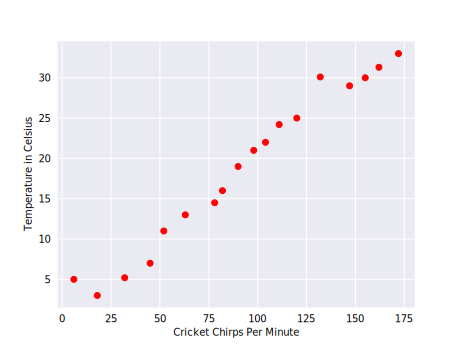
\includegraphics[width=0.8\textwidth]{images/CricketPoints.png}
    
\end{itemize}
\end{frame}

\begin{frame}{Linear Regression}
\begin{itemize}
    \item You could draw a single straight line like the following to approximate this relationship between chirps and temperature.

    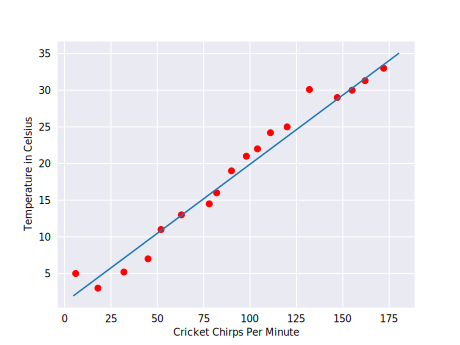
\includegraphics[width=0.8\textwidth]{images/CricketLine.png}
    
\end{itemize}
\end{frame}

\begin{frame}{Linear Regression}
\begin{itemize}
    \item The line doesn't pass through every dot, but the line does clearly show the relationship between chirps and temperature. 
    \item Using the equation for a line, you could write down this relationship as follows:
    
    $$y = m x + b$$
    where:
    \begin{itemize}
        \item $y$ is the temperature in Celsius—the value we're trying to predict.
        \item $m$ is the slope of the line.
        \item $x$ is the number of chirps per minute—the value of our input feature.
        \item $b$ is the y-intercept.
    \end{itemize}
\end{itemize}
\end{frame}

\begin{frame}{Linear Regression}
\begin{itemize}
    \item By convention in ML, you'll write the equation for a model slightly differently:
    $$y' = b + w_1 x_1$$
    where:
    \begin{itemize}
        \item $y$ is the predicted label (a desired output).
        \item $b$ is the bias (the $y$-intercept), sometimes referred to as $w_0$.
        \item $w_1$ is the weight of feature $1$. Weight is the same concept as the ``slope'' $m$ in the traditional equation of a line.
        \item $x_1$ is a feature (a known input).
    \end{itemize}
\end{itemize}
\end{frame}

\begin{frame}{Linear Regression}
\begin{itemize}
    \item To {\bf infer} (predict) the temperature $y'$ for a new chirps-per-minute value $x_1$, just substitute the $x_1$ value into this model.
    
    \item Although this model uses only one feature, a more sophisticated model might rely on multiple features, each having a separate weight $w_1$, $w_2$, etc. 
    
    \item For example, a model that relies on three features might look as follows:
    $$ y' = b + w_1 x_1 + w_2 x_2 + w_3 x_3 $$
\end{itemize}
\end{frame}

\begin{frame}{Key Terms}
\begin{itemize}
    \item bias
    \item inference
    \item linear regression
    \item weight
\end{itemize}
\end{frame}


\subsection{Training and Loss}

\begin{frame}{Training and Loss}
\begin{itemize}
    \item {\bf Training} a model simply means learning (determining) good values for all the weights and the bias from labeled examples. 
    
    \item In supervised learning, a machine learning algorithm builds a model by examining many examples and attempting to find a model that minimizes loss; this process is called {\bf empirical risk minimization}.
    
    \item Loss is the penalty for a bad prediction. That is, {\bf loss} is a number indicating how bad the model's prediction was on a single example. If the model's prediction is perfect, the loss is zero; otherwise, the loss is greater. 
    
    \item The goal of training a model is to find a set of weights and biases that have low loss, on average, across all examples.
\end{itemize}
\end{frame}

\begin{frame}{Training and Loss}
\begin{itemize}
    \item For example, the figure below shows a high loss model on the left and a low loss model on the right. 
    \begin{itemize}
        \item The arrows represent loss.
        \item The lines represent predictions.
    \end{itemize}
\end{itemize}
\includegraphics[width=\textwidth]{images/LossSideBySide.png}
\end{frame}

\begin{frame}{Training and Loss}
\begin{itemize}
    \item Notice that the arrows in the left plot are much longer than their counterparts in the right plot. Clearly, the line in the right plot is a much better predictive model than the line in the left plot.
    
    \item You might be wondering whether you could create a mathematical function -- a loss function -- that would aggregate the individual losses in a meaningful fashion.
    
    \item The linear regression models we'll examine here use a loss function called {\bf squared loss} (also known as $L_2$ loss). 
\end{itemize}
\end{frame}

\begin{frame}{Training and Loss}
\begin{itemize}
    \item The squared loss for a single example is as follows is the difference between the observation (label) $y$ and the prediction $\hat{y}$. That is:
    
    $$ (y - \hat{y})^2 $$
    
\end{itemize}
\end{frame}

\begin{frame}{Training and Loss}
\begin{itemize}
    \item {\bf Mean square error (MSE)} is the average squared loss per example over the whole dataset. To calculate MSE, sum up all the squared losses for individual examples and then divide by the number of examples:
    
    $$ MSE = \frac{1}{m} \sum_{i=1}^m (y^{(i)} - y^{(i)})^2 $$

    \begin{itemize}
        \item $(\boldsymbol{x}^{(i)},y^{(i)})$ is the example in which
        \begin{itemize}
            \item $\boldsymbol{x}^{(i)}$ is the set of features (for instance, chirps/minute, age, gender) 
            \item $y^{(i)}$ is the label (for instance, temperature).
        \end{itemize}
        \item $y^{(i)}$ is a function of the weights and bias in combination with the set of features $\boldsymbol{x}$.
        \item $m$ is the number of examples
    \end{itemize}
\end{itemize}
\end{frame}

\begin{frame}{Training and Loss}
\begin{itemize}
    \item Although MSE is commonly-used in machine learning, it is neither the only practical loss function nor the best loss function for all circumstances.
\end{itemize}
\end{frame}

\begin{frame}{Key Terms}
    \begin{itemize}
        \item empirical risk minimization
        \item loss
        \item mean squared error
        \item squared loss
        \item training
    \end{itemize}
\end{frame}

\section{Reducing Loss}

\subsection{An Iterative Approach}

\begin{frame}{An Iterative Approach}

\begin{itemize}
    \item You'll learn now how a machine learning model iteratively reduces loss.
    
    \item Iterative learning might remind you of the "Hot and Cold" kid's game for finding a hidden object. 
    
    \item In this game, the "hidden object" is the best possible model. You'll start with a wild guess (``The value of $w_1$ is 0.'') and wait for the system to tell you what the loss is. Then, you'll try another guess (``The value of $w_1$ is 0.5.'') and see what the loss is. 
    \item If you play this game right, you'll usually be getting warmer. The real trick to the game is trying to find the best possible model as efficiently as possible.
\end{itemize}

\end{frame}

\begin{frame}{An Iterative Approach}
\begin{itemize}
    \item The following figure suggests the iterative trial-and-error process that machine learning algorithms use to train a model:
\end{itemize}
\includegraphics[width=\textwidth]{images/GradientDescentDiagram.png}
\end{frame}

\begin{frame}{An Iterative Approach}
\begin{itemize}
    
    \item Iterative strategies are prevalent in machine learning, primarily because they scale so well to large data sets.

    \item The ``model'' takes one or more features as input and returns one prediction $y'$ as output. 
    
\end{itemize}
\end{frame}

\begin{frame}{An Iterative Approach}
\begin{itemize}
    \item To simplify, consider a model that takes one feature and returns one prediction:

    $$ \hat{y} = b + w_1 x_1 $$
    
    \item What initial values should we set for $b$ and $w_1$? For linear regression problems, it turns out that the starting values aren't important. We could pick random values, but we'll just take the following trivial values instead:
    
    $$ b = 0\,, \quad w_1 = 0 $$

\end{itemize}
\end{frame}

\begin{frame}{An Iterative Approach}
\begin{itemize}
    \item Suppose that the first feature value is 10. Plugging that feature value into the prediction function yields:

    $$ \hat{y} = 0 + 0 \cdot 10 = 0 $$

    \item The ``Compute Loss'' part of the diagram is the loss function that the model will use. Suppose we use the squared loss function. The loss function takes in two input values:
    \begin{itemize}
        \item $\hat{y}$: The model's prediction for features $\boldsymbol{x}$
        \item $y$: The correct label corresponding to features $\boldsymbol{x}$.
    \end{itemize}
\end{itemize}
\end{frame}

\begin{frame}{An Iterative Approach}
\begin{itemize}
    \item At last, we've reached the ``Compute parameter updates'' part of the diagram. 
    \item It is here that the machine learning system examines the value of the loss function and generates new values for $b$ and $w_1$. 
    \item For now, just assume that this mysterious box devises new values and then the machine learning system re-evaluates all those features against all those labels, yielding a new value for the loss function, which yields new parameter values. 
    \item The learning continues iterating until the algorithm discovers the model parameters with the lowest possible loss. 
    \item Usually, you iterate until overall loss stops changing or at least changes extremely slowly. When that happens, we say that the model has {\bf converged}.
\end{itemize}
\end{frame}

\begin{frame}{Key Point}
\begin{itemize}
    \item A Machine Learning model is trained by starting with an initial guess for the weights and bias and iteratively adjusting those guesses until learning the weights and bias with the lowest possible loss.
\end{itemize}
\end{frame}

\begin{frame}{Key Terms}
\begin{itemize}
    \item convergence
    \item loss
    \item training
\end{itemize}
\end{frame}

\subsection{Gradient Descent}

\begin{frame}{Gradient Descent}
\begin{itemize}
    \item The iterative approach diagram contained a green hand-wavy box entitled ``Compute parameter updates.'' We'll now discuss the underlying algorithms in detail.
    
    \item Suppose we had the time and the computing resources to calculate the loss for all possible values of $w_1$. 
    
\end{itemize}
\end{frame}

\begin{frame}{Gradient Descent}
\begin{itemize}
    \item For the kind of regression problems we've been examining, the resulting plot of loss vs.~$w_1$ will always be convex. In other words, the plot will always be bowl-shaped, kind of like this: 
\end{itemize}
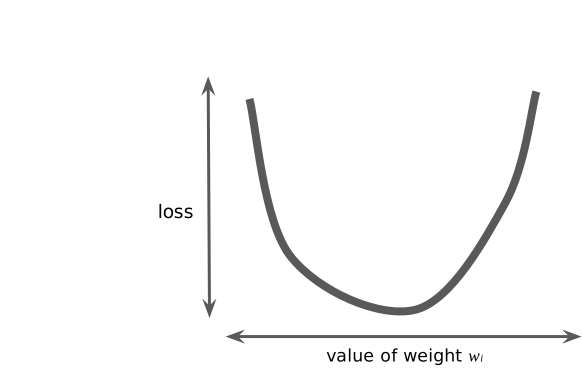
\includegraphics[width=0.9\textwidth]{images/convex.png}
\end{frame}

\begin{frame}{Gradient Descent}
\begin{itemize}
    \item Convex problems have only one minimum; that is, only one place where the slope is exactly $0$. That minimum is where the loss function converges.
    
    \item Calculating the loss function for every conceivable value of  over the entire data set would be an inefficient way of finding the convergence point. 
    
    \item Let's examine a better mechanism—very popular in machine learning—called {\bf gradient descent}.
\end{itemize}
\end{frame}

\begin{frame}{Gradient Descent}
\begin{itemize}
    \item The first stage in gradient descent is to pick a starting value for $w_1$. The starting point doesn't matter much; therefore, many algorithms simply set $w_1$ to $0$ or pick a random value. 
\end{itemize}
\includegraphics[width=0.9\textwidth]{images/GradientDescentStartingPoint.png}
\end{frame}

\begin{frame}{Gradient Descent}
\begin{itemize}
    \item The gradient descent algorithm then calculates the gradient of the loss curve at the starting point. 
    
    \item In the previous figure, the gradient of loss is equal to the derivative (slope) of the curve, and tells you which way is ``warmer'' or ``colder.'' 
    
    \item When there are multiple weights, the gradient is a vector of partial derivatives with respect to the weights.
    
    \item Note that a gradient is a vector, so it has both of the following characteristics:
    \begin{itemize}
        \item a direction
        \item a magnitude
    \end{itemize}
\end{itemize}
\end{frame}

\begin{frame}{Gradient Descent}
\begin{itemize}
    \item The gradient always points in the direction of steepest increase in the loss function. The gradient descent algorithm takes a step in the direction of the negative gradient in order to reduce loss as quickly as possible.
\end{itemize}
\includegraphics[width=0.9\textwidth]{GradientDescentNegativeGradient.png}
\end{frame}

\begin{frame}{Gradient Descent}
\begin{itemize}
    \item To determine the next point along the loss function curve, the gradient descent algorithm adds some fraction of the gradient's magnitude to the starting point as shown in the following figure:
\end{itemize}
\includegraphics[width=0.9\textwidth]{GradientDescentGradientStep.png}
\end{frame}


\begin{frame}{Gradient Descent}
\begin{itemize}
    \item When performing gradient descent, we generalize the above process to tune all the model parameters simultaneously. 
    
    \item For example, to find the optimal values of both $w_1$ and the bias $b$, we calculate the gradients with respect to both $w_1$ and $b$. 
    
    \item Next, we modify the values of $w_1$ and $b$ based on their respective gradients. 
    \item Then we repeat these steps until we reach minimum loss.
\end{itemize}
\end{frame}


\begin{frame}{Key Terms}
\begin{itemize}
    \item gradient
    \item gradient descent
    \item step
\end{itemize}
\end{frame}


\subsection{Learning Rate}

\begin{frame}{Learning Rate}
\begin{itemize}
    \item The gradient vector has both a direction and a magnitude. 
    \item Gradient descent algorithms multiply the gradient by a scalar known as the learning rate (also sometimes called step size) to determine the next point. 
    \item For example, if the gradient magnitude is $2.5$ and the learning rate is $0.01$, then the gradient descent algorithm will pick the next point $0.025$ away from the previous point.
\end{itemize}
\end{frame}

\begin{frame}{Learning Rate}
\begin{itemize}
    \item {\bf Hyperparameters} are the knobs that programmers tweak in machine learning algorithms. Most machine learning programmers spend a fair amount of time tuning the learning rate. If you pick a learning rate that is too small, learning will take too long:
\end{itemize}
\includegraphics[width=0.9\textwidth]{LearningRateTooSmall.png}
\end{frame}


\begin{frame}{Learning Rate}
\begin{itemize}
    \item Conversely, if you specify a learning rate that is too large, the next point will perpetually bounce haphazardly across the bottom of the well:
\end{itemize}
\includegraphics[width=0.9\textwidth]{LearningRateTooLarge.png}
\end{frame}

\begin{frame}{Learning Rate}
\begin{itemize}
    \item There's a Goldilocks learning rate for every regression problem. The Goldilocks value is related to how flat the loss function is. If you know the gradient of the loss function is small then you can safely try a larger learning rate, which compensates for the small gradient and results in a larger step size.
\end{itemize}
\includegraphics[width=0.9\textwidth]{LearningRateJustRight.png}
\end{frame}

\begin{frame}{Key Terms}
\begin{itemize}
    \item hyperparameter
    \item learning rate
    \item step size
\end{itemize}
\end{frame}

\subsection{Optimizing Learning Rate}

\begin{frame}{Optimizing Learning Rate}
\begin{itemize}
    \item Check out jupyter notebook.
\end{itemize}
\end{frame}

\subsection{Stochastic Gradient Descent}

\begin{frame}{Stochastic Gradient Descent}

\begin{itemize}
    \item In gradient descent, a {\bf batch} is the total number of examples you use to calculate the gradient in a single iteration. 
    \item So far, we've assumed that the batch has been the entire data set. 
    \item But often data sets contain huge numbers of examples with huge numbers of features.
    \item Consequently, a batch can be enormous. A very large batch may cause even a single iteration to take a very long time to compute.
    \item A large data set with randomly sampled examples probably contains redundant data. In fact, redundancy becomes more likely as the batch size grows. 
    \item Some redundancy can be useful to smooth out noisy gradients, but enormous batches tend not to carry much more predictive value than large batches.
\end{itemize}
\end{frame}

\begin{frame}{Stochastic Gradient Descent}

\begin{itemize}
    \item What if we could get the right gradient on average for much less computation? 
    \item By choosing examples at random from our data set, we could estimate (albeit, noisily) a big average from a much smaller one. 
    \item {\bf Stochastic gradient descent (SGD)} takes this idea to the extreme--it uses only a single example (a batch size of 1) per iteration. 
    \item Given enough iterations, SGD works but is very noisy. The term ``stochastic'' indicates that the one example comprising each batch is chosen at random.
\end{itemize}

\end{frame}

\begin{frame}{Reducing Loss}
\begin{itemize}
    \item {\bf Mini-batch stochastic gradient descent (mini-batch SGD)} is a compromise between full-batch iteration and SGD. A mini-batch is typically between $10$ and $1,000$ examples, chosen at random. 
    \item Mini-batch SGD reduces the amount of noise in SGD but is still more efficient than full-batch.
    \item To simplify the explanation, we focused on gradient descent for a single feature. Rest assured that gradient descent also works on feature sets that contain multiple features.
\end{itemize}
\end{frame}

\begin{frame}{Key Terms}
\begin{itemize}
    \item batch
    \item batch size
    \item mini-batch
    \item stochastic gradient descent (SGD)
\end{itemize}

\end{frame}

\end{document}